\chapter{Energy Dynamics for the Non-periodic Simulations}
\label{c_nlin_nonper}

I turn my focus in this chapter to the simulations with non-periodic axial boundary conditions; namely the Dirichlet, Neumann, and Sheath simulations. I showed in Sec.~\ref{s_lin_inst}
that the linear properties of these simulations are rather different from the Periodic simulation and from one another. However, the statistical turbulent properties of the four simulations
are all quite similar (Sec.~\ref{s_stat_exam}). This, combined with the observation that the turbulence in the Periodic simulation self-organizes and drives itself by
nonlinear instability, points to the conclusion that the axial boundary conditions have little affect on the nonlinear instability or the energy dynamics in general. 
Nevertheless, additional supporting evidence for this claim can provide confirmation regarding the robustness of the nonlinear instability. I therefore explore the energy dynamics of the
non-periodic simulations in this chapter, attempting to differentiate the nonlinear dynamics from the linear ones.


\section{Fourier Decomposing Non-periodic Functions}
\label{s_fourier_decomp}

To my knowledge, nobody has considered the affect of non-periodic axial boundary conditions on this nonlinear instability in a straight magnetic field. But this is a critical extension of the topic
because in the real world, linear plasma devices don't have periodic boundary conditions. Additionally, the nonlinear instability seems to crucially depend on axial wavenumber dynamics, which should
be affected by the axial boundary conditions. It is perhaps surprising then that nobody has taken up this line of research.

On the other hand, it may not be so surprising given that the non-periodicity can cause interpretation issues regarding the linear vs. the nonlinear instability. 
To clarify, in the periodic case, the linear eigenmodes are sinusoildal with
integer axial mode numbers. And all of the unstable eigenmodes have $|n| \ge 1$. So any energy injection into $n=0$ fluctuations is a clear indication that the unstable linear eigenmodes are not
responsible for such injection. In the non-periodic cases, the linear eigenmodes are not necessarily sinusoidal (see Fig.~\ref{lin_all_gamma} b)) and if they are, they certainly don't have
integer mode numbers. Fourier decompositions of the non-periodic unstable eigenmodes yields finite $n=0$ Fourier coefficients. This can muddle interpretation of energy injection into $n=0$
fluctuations during the turbulent simulation phase. It seems as though a linear eigenmode decomposition may fix this problem, but these decompositions are difficult to perform in practice,
and more importantly, decompositions with highly non-normal bases aren't guaranteed to yield interpretable results. So I proceed with the spectral energy dynamics on non-periodic simulations
and show that the results are less clear-cut than those of the Periodic simulation, but nevertheless, rather conclusive in that the nonlinear instability still dominates.

\begin{figure}[!ht]
\centerline{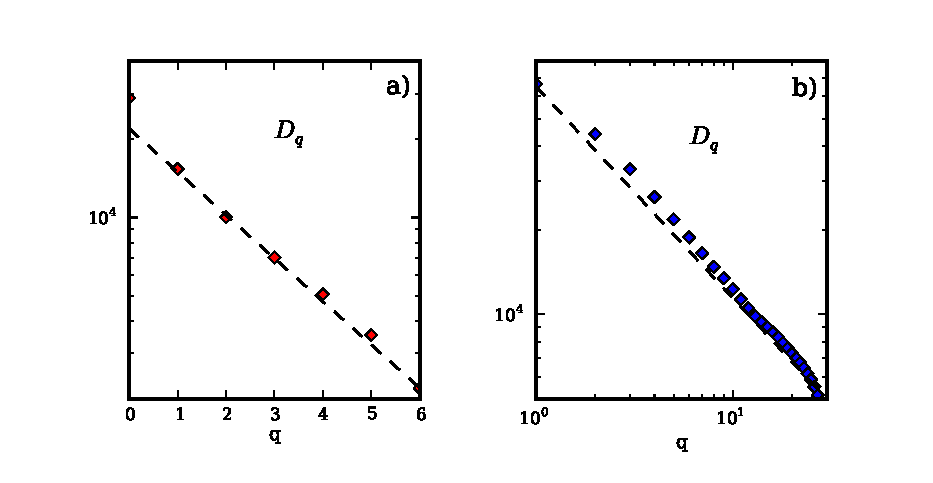
\includegraphics[]{fourier_convergence}}
\caption{Convergence of Fourier reconstructions}
\label{fourier_convergence}
\end{figure}

First, however, I raise another problem regarding spectral energy dynamics and spectral analysis in general. That problem is Gibbs phenomena.
Fourier basis functions are continuous and periodic, so Fourier decomposing
discontinuous or non-periodic functions leads to Gibbs phenomena. One of the significant results of this is the slow convergence of Fourier reconstructions to the original signal.
Mathematically, I can take a discrete signal with the following Fourier decomposition:

\beq
\label{f_decomp}
f(x) = \sum_{k=-Q}^{Q} \hat{f}_k e^{2 \pi i k x},
\eeq

where the $\hat{f}_k$ are ordered in the sum by the size of their absolute value with $\hat{f}_0$ being the largest Fourier coefficient. The Fourier reconstruction of order $q<Q$ is then:

\beq
\label{f_recon}
g_q(x) = \sum_{k=-q}^{q} \hat{f}_k e^{2 \pi i k x}
\eeq

There are several types of convergences of the $g_q$, one of which is the $L1$ norm. Defining the difference between the original signal and the Fourier reconstruction of order $q$ as
$D_q = \sum_x |f(x) - g_q(x)|$, I can look at the convergence of $D_q$ as a function of $q$. For continuous periodic signals, $D_q$ converges exponentially, while it only converges algebraically
(power law) for non-periodic or discontinuous signals. 

As an example, I have plotted $D_q$ for the Periodic and Sheath simulations in Fig.~\ref{fourier_convergence}. The Periodic simulation in Fig.~\ref{fourier_convergence} a) converges exponentially,
while the Sheath simulation in Fig.~\ref{fourier_convergence} b) converges algebraically. Now in this figure, even though the x-axis label $q$ indicates the mode with the $q^{th}$ largest amplitude
by construction of Eq.~\ref{f_recon}, it also happens to correspond to the axial mode number $n$ for all but the last few $q$. In other words, in both simulations, most of the energy is contained
in $n=0$ modes followed by $n=1$ modes and so on. So I should still be able to focus on the $n=0$ and $n = \pm 1$ mode numbers in the energy dynamics data, but they will not contain as much
of the dynamics as they do for the Periodic case.



\section{Energy Dynamics Results}
\label{s_nonper_en_dyn}

\begin{figure}[!ht]
\centerline{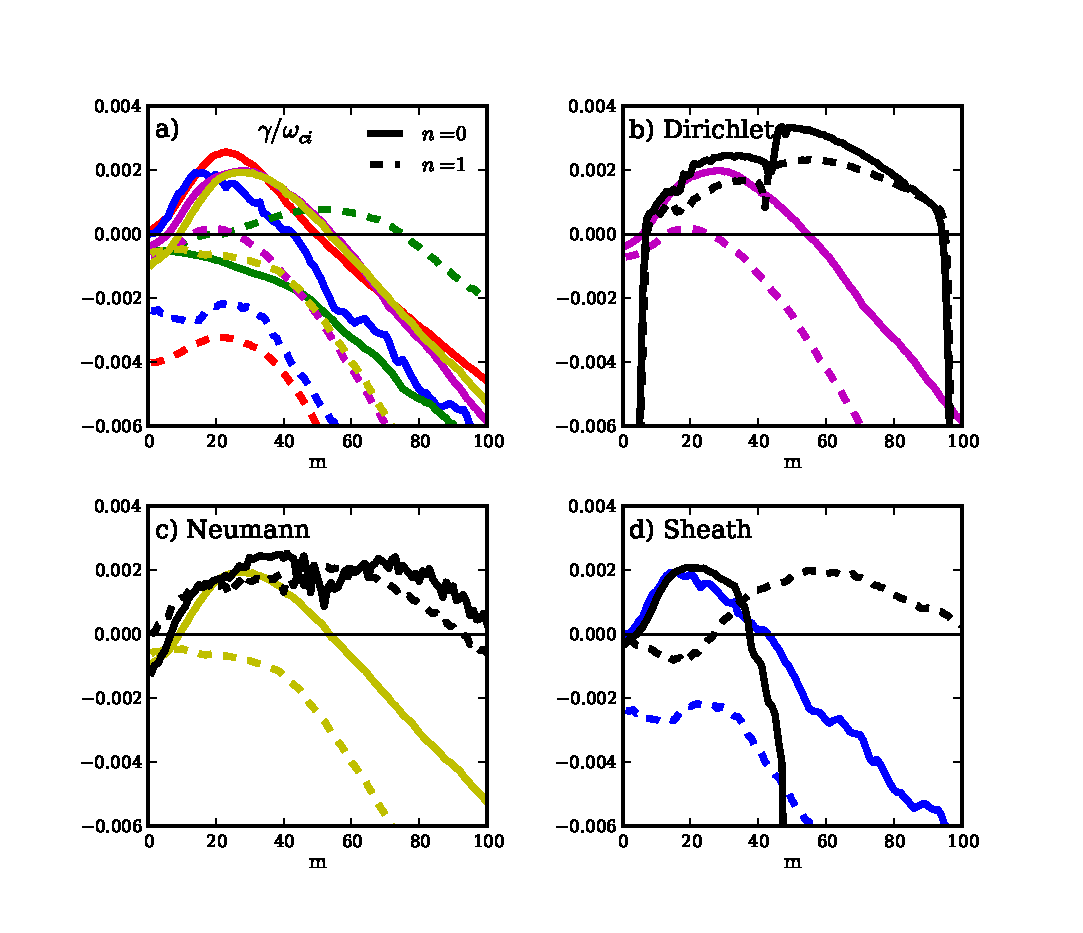
\includegraphics[]{all_gamma}}
\caption{Linear and nonlinear growth rates of all simulations}
\label{all_gamma}
\end{figure}

The simplest way to view the vast quantities of energy dynamics information is through the effective growth rate defined in Eq.~\ref{gamma_def}. So in Fig.~\ref{all_gamma}, I show the growth
rates for all of the simulations. In Fig.~\ref{all_gamma} a), I plot the growth rates during the turbulent phases of all five simulations (see Fig.~\ref{n_statistics} for the color code).
Again, I break up the $n=0$ and $n=1$ components and don't show the $n \ge 2$ growth rates. Notice that the Periodic, Dirichlet, Neumann, and Sheath simulations all have quite similar growth
rates, especially at $n=0$. Their $n=1$ growth rates have similar $m$ dependencies, but somewhat different magnitudes, and the $n=1$ growth rates are all negative except for a small region
in the Dirichlet curve, which is marginal. Contrast these with the $n=0$ suppressed simulation, which recall, is dominated by the linear instability. These growth rates certainly indicate
that the same kind of processes occur for the four similar simulations regardless of axial boundary conditions -- namely, the nonlinear instability process. This isn't too surprising given
the similarity of the turbulent statistics of the four simulations (Fig.~\ref{n_statistics}).

It is also instructive to compare the nonlinear turbulent growth rates against the linear growth rates as I did for the Periodic simulation in Fig.~\ref{lin_per_non0_gamma}. I do this for
the non-periodic simulations in Figs.~\ref{all_gamma} b)-d). The black curves in these figures are the linear growth rates for each respective simulation. For example, the solid black line in
Fig.~\ref{all_gamma} b) corresponds to the $n=0$ linear growth rate of the Dirichlet simulation. The dashed black line in this figure corresponds to the $n=1$ growth rate of the Dirichlet simulation.
Note that the linear growth rates come from the same data as that used in Fig.~\ref{lin_all_gamma}, but these are decomposed in $m$ and $n$, while those were simply decomposed in $m$.

Now all three of these simulations (Dirichlet, Neumann, and Sheath) have a lot of similarity, especially the Dirichlet and Neumann simulations. The $n=1$ growth
rate curves for all three simulations are all qualitatively different between the linear and the nonlinear stage. For the most part, the $n=1$ linear growth rates are always positive, while
the $n=1$ nonlinear growth rates are always negative. The $n=0$ linear growth rates for the Dirichlet and Neumann simulations are similar to the $n=1$ linear growth rates because the linear
eigenmode structures contain roughly equal parts $n=0$ and $n=1$ and the density-potential phases are set by the linear drift-wave physics. The $n=0$ and $n=1$ Sheath simulation linear
growth rates are quite different because the linear eigenmodes actually undergo a bifurcation at $m \sim 40$. All $m <40$ Sheath linear eigenmodes have shapes like that in Fig.~\ref{lin_all_gamma} b),
which are even about the axial midpoint. However, all $m>40$ linear eigenmodes have shapes that are odd about the axial midpoint. The CWM has even and odd solution branches whose growth rates
cross at $m \sim 40$, causing this seemingly odd behavior.

In any case, it is interesting that the $n=0$ linear and nonlinear
growth rates for these three simulations are nearly equal for $m<50$. However, they are not at all similar for $m>50$. Does this low $m$ region of similarity indicate that the linear instability
dominates these simulations? Based on Fig.~\ref{all_gamma} a), the $m>50$ region, and the $n=1$ dissimilarity, I would say that the nonlinear instability is still the dominant player. However, it's
not conclusive either way, and it's possible that in some complicated way, the linear and nonlinear physics are somewhat similar in this region. This is the problem of using Fourier decompositions
rather than linear eigenmode decompositions, although as I stated before, there's no guarantee that an eigenmode decomposition would yeild anything more conclusive because of the eigenmode
nonorthogonality. Eigenmode nonorthogonality is the real culprit to all of the difficulties, in fact. It causes the nonlinear instability, but it also makes it difficult to identify in some cases.
Therefore, I try to devise a way around this in the next section.

\section{Linear vs Nonlinear Structure Correlation}
\label{s_lin_vs_nlin_struc}

To try to sort out the problem of linear vs. nonlinear instability in a non-normal linear system, I propose the following method.
First, imagine the case where a simulation is dominated by a linear instability. Then, the fastest growing linear
eigenmode dominates the system, nonlinearly transfering some energy to more weakly unstable or even stable eigenmodes. In this case, a large portion of the energy should remain in the fastest
growing linear eigenmode~\cite{hatch2011}. In the alternative case where a nonlinear instability is dominant, 
the linear eigenmode should have little bearing on the structure of the turbulence and therefore little
energy should be contained in this eigenmode. Therefore, a reasonable gauge of whether a linear or nonlinear instability dominates a system is the fraction of energy in a turbulent system
that is contained in the fastest growing linear eigenmode. This may be calculated by projecting the fastest growing eigenmode onto the turbulent state.

Formally, in my model, I fully describe the turbulent state by four independent fields, which I can appended into a single vector of the spatio-temporal field functions: 
$\bm{f}_{turb}(\vec{r},t) = \{N(\vec{r},t),T_e(\vec{r},t),\gradperp \phi(\vec{r},t), \vpe(\vec{r},t)\}$. This vector may be decomposed in a complete basis:

\beq
\label{basis_decomp}
\bm{f}_{turb}(\vec{r},t) = \sum_{i,m} c_{i,m}(t) \bm{\psi}_{i,m}(r,z) e^{i m \theta},
\eeq

where $\bm{\psi}_{i,m}(r,z)$ are time-independent spatial complex basis functions of the form $\bm{\psi}_{i,m}(r,z) = \left\{ n_{i,m}(r,z),t_{i,m}(r,z),\gradperp \phi_{i,m}(r,z), v_{i,m}(r,z) \right\}$,
and $c_{i,m}(t)$ are the complex time-dependent amplitudes. I have explicitly imposed a Fourier bases for the $\theta$ dependence of the basis functions. The total number of
linearly independent basis functions is the number of total grid points used in the simulation times the number of independent fields, which is four in this case.
Now, $\bm{\psi}_{i,m}(r,z)$ can be any linearly independent set of functions and need not be the linear eigenfunctions
of the system. In fact, I want to use orthogonal basis functions, ruling out the linear eigenfunctions.
However, it is quite useful to set $\bm{\psi}_{0,m}(r,z)$ to the fastest
growing linear eigenmode because this is the structure of interest that is to be projected onto the turbulence. 
The other $\bm{\psi}_{i \ne 0,m}(r,z)$ comprise the remainder of the orthonormal basis, and they must be different from
the remaining linear eigenfunctions in order to complete the orthogonal basis. It isn't necessary for the purpose of this study to actually compute these other basis functions, but if I were to compute
them, I would probably start with all of the linear eigenmodes
and perform a Gram-Schmidt orthogonalization procedure, making sure to start with the fastest growing eigenmode in order to preserve it. Using this procedure, Hatch et al.~\cite{hatch2011}
found that a significant fraction ($\sim 50\%$) of the energy in a turbulent state of ITG turbulence was contained in the fastest growing linear eigenmode at each perpendicular wavenumber.
Such a result, however, doesn't require knowledge of the other basis functions, and thus I don't compute them here.

Now, to compute the fraction of energy in the fastest growing eigenmode to the total energy, 
I first define an inner product that is energetically meaningful and that sets the orthonormality of the basis functions:

\beq
\label{basis_orthonormality}
\left< \bm{\psi}_{i,m},\bm{\psi}_{j,m} \right> = \int w \bm{\psi}_{i,m}^* \cdot \bm{\psi}_{j,m} dV = \delta_{i,j}.
\eeq

The weighting $w$ is such that $\left< \bm{f}_{turb}, \bm{f}_{turb} \right> = E_{turb}$.
Now from Eqs.~\ref{basis_decomp} and~\ref{basis_orthonormality}, $\left< \bm{f}_{turb}, \bm{f}_{turb} \right> = E_{turb} = \sum_{i,m} |c_{i,m}|^2$ and 
$\left< f_{turb,m}, f_{turb,m} \right> = E_{turb,m} = \sum_i |c_{i,m}|^2$.
Then, the amount of energy contained in the fastest growing mode (for each $m$) is given by the square of the projection
of the mode onto the turbulence: $E_{0,m} = \left| \left< \bm{\psi}_{0,m}, f_{turb,m} \right> \right|^2 = |c_{0,m}|^2$. The ratio 
$R_m = E_{0,m}/E_{turb,m}$ is a measure of the fraction of turbulent energy contained in the fastest growing linear eigenmode. 

Of course, $E_{turb,m}$ is easily calculated from the turbulent state, but $E_{0,m}$ in the 
turbulent state can only be found with knowledge of the fastest growing eigenfunction. The fastest growing eigenfunction, though, can be found easily by running a simulation from a random 
or turbulent state with all of the nonlinearities removed from the model equations. After some time, the fastest growing eigenfunctions will come to
dominate the fluctuation structure. Then, a Fourier decomposition in $m$ space will separate the fastest growing eigenfunctions at each $m$, including the real and imaginary part
of the eigenfunctions (up to a time dependent complex constant, which is removed by normalizing the eigenfunction). I can then project the eigenfunctions onto the turbulent state
with the inner product defined in Eq.~\ref{basis_orthonormality}, giving $E_{0,m}$.

I do this and show the ratio $R_m$ in Fig.~\ref{lin_to_nl_ratios} for the five simulations. 
For the most part, the simulations other than the $n=0$ suppressed one have a small value of the ratio ($R_m < 0.3$) for all $m$. 
This confirms that the turbulence largely self-organizes without regard to the linear physics in the four other simulations. 
The one exception is the Dirichlet simulation for $m > 50$, which has $R_m \sim 0.5$. This is quite the unexpected result, and I can't explain it based on any of the other evidence.
Most of the energy in this and the other simulations, however, 
is at low $m$ (Fig.~\ref{energy_spectra}), so these larger $m$ eigenmodes don't make a large impact on the overall structure of the turbulence.

In fact, $R_m$ is below $0.1$ for $m<40$ for the periodic, Dirichlet, and Neumann simulations, precisely the area where
$n=0$ structures dominate the energy spectrum. This answers the question posed in the previous section regarding the similarity in the $n=0, m<40$ linear and nonlinear growth rates
for the Dirichlet and Neumann simulations. The fastest growing linear eigenmodes do not significantly drive the turbulence in this region. The nonlinear instability does.

On the other hand, the fastest growing eigenfunctions make up a significant fraction of the energy in the $n=0$ suppressed simulation. Where the linear drift wave instability 
(and the turbulent growth rate) is the strongest (at $m \sim 50$), $R_m \sim 0.5$. The linear physics controls the $n=0$ suppressed simulation, and the linear eigenmode structure certainly asserts itself
in the turbulence, but only to a degree ($50\%$).

The Sheath simulation is the most difficult to analyze because it has more linear eigenmode dominance at low $m$ than the other simulations. $R_m$ is still only about $0.25$ there. While this isn't
at the level of the $n=0$ suppressed simulation or the Hatch et al. gyrokinetic ITG simulation~\cite{hatch2011}, it still might be significant. It appears that the linear instability
never completely disappears from any of the simulations, and the level to which it acts on the turbulence differs between the different simulations. The Sheath simulation is driven more by
its linear instability than all of the others except for the $n=0$ suppressed simulation, indicating a possibly important role for the CWM in LAPD, though LAPD doesn't have such simple
boundary conditions. However, the turbulence statistics of the Sheath simulation are so similar to those of the other simulations (Sec.~\ref{s_stat_exam}) that $R_m \sim 0.25$ probably
isn't significant enough to say that the linear instability dominates.


\begin{figure}[!ht]
\centerline{\includegraphics[]{lin_to_nl_ratios}}
\caption{Energy fraction contained in the most unstable eigenmodes}
\label{lin_to_nl_ratios}
\end{figure}



\section{Nonlinear Saturation Levels}
\label{ss_nl_sat_levels}

A common topic of plasma turbulence is the prediction of the saturation level of turbulence. Generally, such predictions are based off of linear properties, however, a dominant nonlinear
instability should have an affect on the level at which the turbulence saturates. One theory -- mixing length theory -- based on linear drift waves predicts that the saturation level should
be about $\gamma/k_\perp^2$ where $\gamma$ and $k_\perp$ are the growth rate and perpendicular wavenumber of the fastest growing linear eigenmode~\cite{horton1990}. Turbulence driven
by a nonlinear instability may saturate at some other level, which seems probable given Fig.~\ref{n_statistics}, which shows that the $n=0$ suppressed simulation saturates
at a lower level than the simulations driven by the nonlinear instability.

Mixing length theory provides an estimate for the turbulence saturation level where only properties of the linear eigenmodes are known. This can be quite useful to find scaling relations, and allows
prediction without direct numerical simulation. Therefore, I develop a corresponding estimate based on the drift wave turbulence driven by the nonlinear instability that I have described.
Now, it is quite difficult to predict a saturation level based on a nonlinear mechanism when nonlinear simulation results are not available. However, as suggested in Ref.~\cite{cheng1979},
and as seen in Fig.~\ref{rms_evolution} b), it appears that the turbulence begins to saturate when the amplitude of the $n=0$ field components becomes equal to the $n=1$ field components.
At this point, the strongest nonlinear interaction term catches up to the linear terms, bringing about the onset of saturation. However, the nonlinear instability really doesn't become important
up until this point, which is why saturation occurs only when values are a few times higher than this point. Therefore, this crossing point can only be seen as a rough approximation for the
saturation level, and more work will be needed to improve upon this calculation.

Now in order to find the crossing point amplitude, notice from Fig.~\ref{rms_evolution} b), that before the components become equal, in the linear phase of the simulation,
the $n=0$ components seem to have twice the growth rate of the $n=1$ components. This indicates that the
$n=0$ components are driven nonlinearly (parametrically). Furthermore, both are exponentially growing in the linear phase. It is possible then to use only linear eigenmode knowledge
to compute the level at which the $n=0$ and $n=1$ components become equal as long as both start at small amplitudes and experience a few e-foldings before saturating. To find the crossing
point, I first derive an expression for the time evolution of the linear eigenmode amplitudes. According to Drazin~\cite{drazin1981}, such an evolution for the linear eigenmode $A_j$
should take the form:

\beq
\label{drazin_form}
\diff{A_j}{t} =  s_j A_j + N_j(A_k)
\eeq
where the complex function $N_j$ of the $A_k$s represents the nonlinear action of all the $k$ modes on the $j$th (including the self-interaction). I now derive such an equation for my model
set, finding the explicit forms for $s_j$ and $N_j$.

\subsection{Linear Eigenvector Amplitude Evolution}
\label{ss_eigenmode_ev}

The linear eigenvectors are fixed composit objects of the independent fields ($N, \vpe, \phi$ and $T_e$). Each one has a fixed complex-valued spatial structure where the different fields have
a certain amplitude and phase relationship between each other. Each one evolves in time under the linear equation set with a fixed frequency and growth rate. Eigenmode structures of global
simulations have radial and axial shapes that are not described by well-known functions like sines and cosines or Bessel functions. So to simplify matters, 
I use a local model in which each linear eigenmode can simply be identified by its wavevector $\vec{k} = (k_r, k_\theta, k_z)$. Then number of eigenvectors at each
$\vec{k}$ is equal to the number of fields -- 4 in my case.

Formally, the local fully spectral version of Eqs.~\ref{ni_eq}-~\ref{te_eq} can be written as

\beq
\label{vec_eqns}
\pdiff{\bm{\xi}_{\vec{k}}}{t} = {\bf M}_{\vec{k}} \cdot \bm{\xi}_{\vec{k}} + \sum_{\vec{k'}} (k_r k'_\theta - k'_r k_\theta) \bm{\xi}_{\vec{k'}} \phi_{\vec{k}-\vec{k'}},
\eeq
where

\beqar
\label{xi_M_def}
\bm{\xi}_{\vec{k}}  & = & \left( \begin{array}{c} N_{\vec{k}} \\ v_{\para e \vec{k}} \\ \phi_{\vec{k}} \\ T_{e \vec{k}} \end{array} \right), \nonumber \\
{\bf M}_{\vec{k}}  & = & \left( \begin{array}{cccc}   - \mu_N \kperp^2 & -i k_z & -\frac{i k_\theta}{L_N} & 0 \\
-\frac{i k_z m_i}{m_e} & - \nue & \frac{i k_z m_i}{m_e} & -1.71 \frac{i k_z m_i}{m_e} \\
0 & \frac{i k_z}{\kperp^2} & -\nuin \mu_\phi \kperp^2 & 0 \\
0 & -1.71 \frac{2}{3} i k_z & -\frac{i k_\theta}{L_T} & -\frac{2}{3} \kpe k_z^2 - \frac{2 m_e \nue}{m_i} - \mu_T \kperp^2
\end{array} \right) \nonumber
\eeqar
where I have used $\pdr N_0 = -1/L_N$ in accordance with the local approximation, and I have neglected the sources, which are only nonzero for $k_r = k_\theta = 0$ in any case.
The final term on the RHS is the nonlinear advection contribution. Without this, the system is linear, constituting a linear eigenvalue problem:

\beq
\label{lin_eval_problem}
\pdiff{\bm{\rho}_{\vec{k},j}}{t} = -i \omega_{\vec{k},j} = {\bf M}_{\vec{k}} \cdot \bm{\rho}_{\vec{k},j}
\eeq
where $\omega_{\vec{k},j}$ and $\bm{\rho}_{\vec{k},j}$ are the eigenvalues and eigenvectors of ${\bf M}_{\vec{k}}$. $j$ is an index that goes from 1 to 4, 
since there are 4 linear independent eigenvectors for each $\vec{k}$. I note that the linear matrix
${\bf M}_{\vec{k}}$ is not normal; therefore, the eigenvectors are not orthogonal. This can be a problem for eigenvector decompositions. However, the \emph{left} eigenvectors
are orthogonal to the right eigenvectors: ${\bf l}_{\vec{k},i}^T \bm{\rho}_{\vec{k},j} = \delta_{i,j}$, where

\beq
\label{left_eigvecs}
{\bf l}_{\vec{k},i}^T \cdot {\bf M}_{\vec{k}} = -i \omega_{\vec{k},j} {\bf l}_{\vec{k},i}^T.
\eeq

Now decomposing the spectral vectors $\bm{\xi}_{\vec{k}}$ with the linear eigenvectors:

\beq
\label{eigendecomp}
\bm{\xi}_{\vec{k}} = \sum_{j=1}^4 A_{\vec{k},j} \bm{\rho}_{\vec{k},j}
\eeq
where $A_{\vec{k},j}$ are the time-dependent eigenmode amplitude coefficients, I substitute this decomposition into Eq.~\ref{vec_eqns}:

\beq
\label{vec_eqns_sub}
\sum_j \bm{\rho}_{\vec{k},j} \pdiff{A_{\vec{k},j}}{t} = \sum_j A_{\vec{k},j} {\bf M}_{\vec{k}} \cdot \bm{\rho}_{\vec{k},j} + \sum_{\vec{k'},j} A_{\vec{k'},j} (k_r k'_\theta - k'_r k_\theta) \bm{\rho}_{\vec{k'},j} \phi_{\vec{k}-\vec{k'}}.
\eeq

Contracting this equation on the left by the left eigenvector $l_{\vec{k},i}$ and using the eigenvector orthogonality gives

\beq
\label{eigenmode_evolution}
\diff{A_{\vec{k},i}}{t} = - i \omega_{\vec{k},i} A_{\vec{k},i} + \sum_{k'} A_{\vec{k'},i} (k_r k'_\theta - k'_r k_\theta) \phi_{\vec{k}-\vec{k'}}.
\eeq

This has the Drazin form of Eq.~\ref{drazin_form} with $s_j$ as the complex linear eigenfrequencies and the $N_j$ as a form indicative of three-wave interactions from nonlinear advection. With this,
I proceed to find the amplitude at which the $n=0$ eigenmodes cross with the $n=1$ eigenmodes.

\subsection{Mixing Length Approximation}
\label{ss_mixing_length}

To begin, I apply Eq.~\ref{eigenmode_evolution} to the fastest growing drift wave in the linear phase of the simulation before the $n=0 / n=1$ crossing.
The $n=1$ fastest growing eigenmode curve, which has $m \sim 60$, evolves as:

\beq
\label{dw_evolution1}
\diff{A_d}{t} = - i \omega_d A_d
\eeq

where $A_d$ represents the fastest growing $n=1, m \sim 60$ linear drift wave structure with time-dependent amplitude ($d$ is shorthand for the wavevector of this eigenmode). 
Note that I have made the assumption that in the linear phase of the simulation, the linear term
dominates the nonlinear term, which is quadratic in two small quantities. The solution of this equation is:

\beq
\label{dw_evolution2}
A_d(t) = A_d(0) e^{- i \omega_d t}.
\eeq

On the other hand, the $n=0$ mode has much smaller amplitude than the linear drift wave during the linear simulation phase, meaning that the nonlinear term can be comparable to or larger than
the linear term. Specifically, the evolution equation for the $n=0$ ``convective cells'' is:

\beq
\label{cc_evolution1}
\diff{A_c}{t} = - i \omega_c A_c + \sum_{\vec{k'}} (k_{rc} k'_\theta - k'_r k_{\theta c}) A_{\vec{k'}} \phi_{c - \vec{k'}}.
\eeq

Now, the convective cells that nonlinearly grow the fastest have $m \sim 0$. This is clear by noting that the largest term in the sum should have $\vec{k'} = d$ and $c \sim 0$. 
Using the symbol $M_{c d}$ for the wavevector difference $k_{r c} k_{\theta d} - k_{r d} k_{\theta c}$ and noting that $\phi_{-d} = \phi^*_d \sim A_d^*$,

\beq
\label{cc_evolution2}
\diff{A_c}{t} \approx - i \omega_c A_c + M_{c d} |A_d|^2.
\eeq

Plugging in Eq.~\ref{dw_evolution2} into the $A_d$ in this equation, and then solving this differential equation for $A_C(t)$ results in:

\beq
\label{cc_evolution3}
A_c(t) = A_c(0) e^{- i \omega_c t} + \frac{M_{c d} |A_d(0)|^2}{2 \gamma_d + i \omega_c} \left( e^{2 \gamma_d t} - e^{- i \omega_c t}  \right).
\eeq

Now a large simplifying approximation is that $\omega_c = 0$. I essentially take the linear eigensystem of these convective cells to have zero axial wavenumber, zero frequency and growth rate, 
near-zero azimuthal wavenumber, and radial wavenumber about twice that of the drift wave radial wavenumber. All of these assumptions are confirmed by the spectra of the convective cells and
drift waves (not shown here). Also, these mean that $k_{r c} k_{\theta d} \gg k_{r d} k_{\theta c}$, so that $M_{c d} \approx k_{r c} k_{\theta d}$ Then,

\beq
\label{cc_evolution4}
A_c(t) = A_c(0) + \frac{k_{r c} k_{\theta d} |A_d(0)|^2}{2 \gamma_d } \left( e^{2 \gamma_d t} - 1  \right).
\eeq

At the time ($t_f$), when the amplitudes of the drift waves and convective cells equal one another, the initial perturbation $A_c(0)$ is much smaller than the second term on the right hand side
of Eq.~\ref{cc_evolution4} and can therefore be neglected when looking at large times. While this doesn't have to be true in general, it is true if the initial perturbations are set small enough.
In fact, if the initial perturbations are not set to be small enough, the convective cells will not necessarily grow nonlinearly before saturating -- they could grow transiently due to the
nonorthogonality of the linear eigenmodes~\cite{camargo1998,cohen2009}.
So, setting the amplitude of $A_d(t_f)$ from Eq.~\ref{dw_evolution2} to the amplitude of 
$A_c(t_f)$ from Eq.~\ref{cc_evolution4} and performing some algebra, the result is:

\beq
\label{dw_cc_scaling}
|A_c(t_f)| = |A_d(t_f)| = \frac{2 \gamma_d}{k_{r c} k_{\theta d}}.
\eeq

The factor of two probably isn't significant given the approximations that went into this result, but the scalings of the drift wave growth rate, the drift wave azimuthal wavenumber,
and the convective cell radial wavenumber are. The result is very similar to the mixing length result except that the wavenumbers of interest are from both the drift waves and the
convective cells rather than from just the drift waves. Putting in LAPD values for this relation gives that the crossing level amplitude should be about $0.05$. This is consistent
with the amplitude at which the simulations begin to saturate, as can be seen in Fig.~\ref{rms_evolution} a). Again, though, the ultimate saturation level is somewhat larger than this,
and it's not clear if that ultimate saturation level can be completely predicted without direct numerical simulation.

One last point I want to make involves the $n \ge 2$ curves in Fig.~\ref{rms_evolution} b). These curves all appear to grow at the same growth rate as the $n=1$ curve during the linear
stage of the simulation. This may seem odd because the linear growth rates of the eigenmodes with these higher axial mode numbers are much less than the growth rate of the fastest
$n=1$ eigenmode. Furthermore, if these modes were to be pumped nonlinearly (parametrically), one might expect them to grow with twice the growth rate of the $n=1$ curve just like the
$n=0$ curve does. In fact, the $n \ge 2$ curves are pumped nonlinearly. A look at the spectra (not shown) reveals that all of the $n \ge 2$ modes have $k_r-k_\theta$ spectra
just like that of the $n=1$ mode. So this means that the nonlinear interaction that drives the $n \ge 2$ modes involves the fastest growing $n=1$ linear eigenmode beating against an eigenmode
that has $k_r \sim k_\theta \sim 0$. This second eigenmode has close to zero growth rate, meaning that the $n \ge 2$ modes will only grow at the same rate as the fastest growing
$n=1$ linear eigenmode and not at twice its growth rate. It's difficult to guess this \emph{a priori} due to the complexity of the nonlinear transfer term, so it seems that simulation
results have to provide the evidence for this.
